\subsubsection{Blending}
\label{sec:blending}

Given $\vec{p}$ and $\vec{x}$.
%
Let $\left\{\hat{p_0},\hat{p_1},\hat{p_2},\hat{p_3}\right\}$ be the simplex cell enclosing the footprint shape $\vec{p}$ with barycentric weights $\vec{a} \in \interval{0}{1}^4$.
%
Then for each grid point $\hat{p_i}$ let $N_{ij}$ denote the meso-facet counts attached to the vertices $\hat{x}_{ij}$ surrounding $\vec{x}_{\hat{p_i}}$ with barycentric weights $\vec{b_i} \in \interval{0}{1}^3$.


% Wrong, when also binomially distributed
% Therefore,
% %
% \begin{equation}
%     N = \sum_{i=0}^{3} a_i \sum_{j=0}^{2} b_{ij} N_{ij}
% \end{equation}
% %
% is the blended meso-facet count inside the pixel footprint.


We want to blend the number of glints between random seeds $\theta_{ijk}$ that we attach to each vertex $\hat{\omega}_k$ framing the half vector $\vec{\omega_h}$ on the tangent plane grid with the bilinear weights being $\vec{c_{ij}} \in \interval{0}{1}^4$.
%
Therefore, we will compare two different blending approaches.

\begin{figure}[!htb]
    \centering
    \begin{subfigure}[b]{0.32\columnwidth}
        \resizebox{1\linewidth}{!}{\input{figures/blending-reference.tikz}}
        \vspace{-5pt}
        \caption{Reference\label{fig:blending-reference}}
    \end{subfigure}
    %
    \begin{subfigure}[b]{0.32\columnwidth}
        \resizebox{1\linewidth}{!}{% This file was created with tikzplotlib v0.10.1.
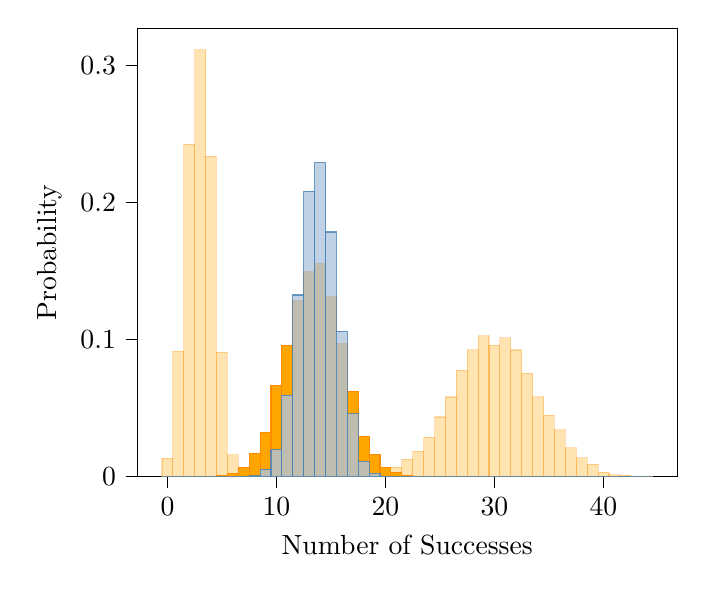
\begin{tikzpicture}

\definecolor{darkgray176}{RGB}{176,176,176}
\definecolor{darkorange}{RGB}{255,140,0}
\definecolor{lightsteelblue}{RGB}{176,196,222}
\definecolor{orange}{RGB}{255,165,0}
\definecolor{steelblue}{RGB}{70,130,180}

\begin{axis}[
tick align=outside,
tick pos=left,
x grid style={darkgray176},
xlabel={Number of Successes},
xmin=-2.75, xmax=46.75,
xtick style={color=black},
y grid style={darkgray176},
ylabel={Probability},
ymin=0, ymax=0.32739,
ytick style={color=black}
]
\draw[draw=darkorange,fill=orange,opacity=0.3] (axis cs:-0.5,0) rectangle (axis cs:0.5,0.0135);
\draw[draw=darkorange,fill=orange,opacity=0.3] (axis cs:0.5,0) rectangle (axis cs:1.5,0.0915);
\draw[draw=darkorange,fill=orange,opacity=0.3] (axis cs:1.5,0) rectangle (axis cs:2.5,0.2428);
\draw[draw=darkorange,fill=orange,opacity=0.3] (axis cs:2.5,0) rectangle (axis cs:3.5,0.3118);
\draw[draw=darkorange,fill=orange,opacity=0.3] (axis cs:3.5,0) rectangle (axis cs:4.5,0.234);
\draw[draw=darkorange,fill=orange,opacity=0.3] (axis cs:4.5,0) rectangle (axis cs:5.5,0.0906);
\draw[draw=darkorange,fill=orange,opacity=0.3] (axis cs:5.5,0) rectangle (axis cs:6.5,0.0158);
\draw[draw=darkorange,fill=orange,opacity=0.3] (axis cs:6.5,0) rectangle (axis cs:7.5,0);
\draw[draw=darkorange,fill=orange,opacity=0.3] (axis cs:7.5,0) rectangle (axis cs:8.5,0);
\draw[draw=darkorange,fill=orange,opacity=0.3] (axis cs:8.5,0) rectangle (axis cs:9.5,0);
\draw[draw=darkorange,fill=orange,opacity=0.3] (axis cs:9.5,0) rectangle (axis cs:10.5,0);
\draw[draw=darkorange,fill=orange,opacity=0.3] (axis cs:10.5,0) rectangle (axis cs:11.5,0);
\draw[draw=darkorange,fill=orange,opacity=0.3] (axis cs:11.5,0) rectangle (axis cs:12.5,0);
\draw[draw=darkorange,fill=orange,opacity=0.3] (axis cs:12.5,0) rectangle (axis cs:13.5,0);
\draw[draw=darkorange,fill=orange,opacity=0.3] (axis cs:13.5,0) rectangle (axis cs:14.5,0);
\draw[draw=darkorange,fill=orange,opacity=0.3] (axis cs:14.5,0) rectangle (axis cs:15.5,0);
\draw[draw=darkorange,fill=orange,opacity=0.3] (axis cs:15.5,0) rectangle (axis cs:16.5,0);
\draw[draw=darkorange,fill=orange,opacity=0.3] (axis cs:16.5,0) rectangle (axis cs:17.5,0);
\draw[draw=darkorange,fill=orange,opacity=0.3] (axis cs:17.5,0) rectangle (axis cs:18.5,0);
\draw[draw=darkorange,fill=orange,opacity=0.3] (axis cs:18.5,0) rectangle (axis cs:19.5,0);
\draw[draw=darkorange,fill=orange,opacity=0.3] (axis cs:19.5,0) rectangle (axis cs:20.5,0);
\draw[draw=darkorange,fill=orange,opacity=0.3] (axis cs:20.5,0) rectangle (axis cs:21.5,0);
\draw[draw=darkorange,fill=orange,opacity=0.3] (axis cs:21.5,0) rectangle (axis cs:22.5,0);
\draw[draw=darkorange,fill=orange,opacity=0.3] (axis cs:22.5,0) rectangle (axis cs:23.5,0);
\draw[draw=darkorange,fill=orange,opacity=0.3] (axis cs:23.5,0) rectangle (axis cs:24.5,0);
\draw[draw=darkorange,fill=orange,opacity=0.3] (axis cs:24.5,0) rectangle (axis cs:25.5,0);
\draw[draw=darkorange,fill=orange,opacity=0.3] (axis cs:25.5,0) rectangle (axis cs:26.5,0);
\draw[draw=darkorange,fill=orange,opacity=0.3] (axis cs:26.5,0) rectangle (axis cs:27.5,0);
\draw[draw=darkorange,fill=orange,opacity=0.3] (axis cs:27.5,0) rectangle (axis cs:28.5,0);
\draw[draw=darkorange,fill=orange,opacity=0.3] (axis cs:28.5,0) rectangle (axis cs:29.5,0);
\draw[draw=darkorange,fill=orange,opacity=0.3] (axis cs:29.5,0) rectangle (axis cs:30.5,0);
\draw[draw=darkorange,fill=orange,opacity=0.3] (axis cs:30.5,0) rectangle (axis cs:31.5,0);
\draw[draw=darkorange,fill=orange,opacity=0.3] (axis cs:31.5,0) rectangle (axis cs:32.5,0);
\draw[draw=darkorange,fill=orange,opacity=0.3] (axis cs:32.5,0) rectangle (axis cs:33.5,0);
\draw[draw=darkorange,fill=orange,opacity=0.3] (axis cs:33.5,0) rectangle (axis cs:34.5,0);
\draw[draw=darkorange,fill=orange,opacity=0.3] (axis cs:34.5,0) rectangle (axis cs:35.5,0);
\draw[draw=darkorange,fill=orange,opacity=0.3] (axis cs:35.5,0) rectangle (axis cs:36.5,0);
\draw[draw=darkorange,fill=orange,opacity=0.3] (axis cs:36.5,0) rectangle (axis cs:37.5,0);
\draw[draw=darkorange,fill=orange,opacity=0.3] (axis cs:37.5,0) rectangle (axis cs:38.5,0);
\draw[draw=darkorange,fill=orange,opacity=0.3] (axis cs:38.5,0) rectangle (axis cs:39.5,0);
\draw[draw=darkorange,fill=orange,opacity=0.3] (axis cs:39.5,0) rectangle (axis cs:40.5,0);
\draw[draw=darkorange,fill=orange,opacity=0.3] (axis cs:40.5,0) rectangle (axis cs:41.5,0);
\draw[draw=darkorange,fill=orange,opacity=0.3] (axis cs:41.5,0) rectangle (axis cs:42.5,0);
\draw[draw=darkorange,fill=orange,opacity=0.3] (axis cs:42.5,0) rectangle (axis cs:43.5,0);
\draw[draw=darkorange,fill=orange,opacity=0.3] (axis cs:43.5,0) rectangle (axis cs:44.5,0);
\draw[draw=darkorange,fill=orange,opacity=0.3] (axis cs:-0.5,0) rectangle (axis cs:0.5,0);
\draw[draw=darkorange,fill=orange,opacity=0.3] (axis cs:0.5,0) rectangle (axis cs:1.5,0);
\draw[draw=darkorange,fill=orange,opacity=0.3] (axis cs:1.5,0) rectangle (axis cs:2.5,0);
\draw[draw=darkorange,fill=orange,opacity=0.3] (axis cs:2.5,0) rectangle (axis cs:3.5,0);
\draw[draw=darkorange,fill=orange,opacity=0.3] (axis cs:3.5,0) rectangle (axis cs:4.5,0);
\draw[draw=darkorange,fill=orange,opacity=0.3] (axis cs:4.5,0) rectangle (axis cs:5.5,0);
\draw[draw=darkorange,fill=orange,opacity=0.3] (axis cs:5.5,0) rectangle (axis cs:6.5,0);
\draw[draw=darkorange,fill=orange,opacity=0.3] (axis cs:6.5,0) rectangle (axis cs:7.5,0);
\draw[draw=darkorange,fill=orange,opacity=0.3] (axis cs:7.5,0) rectangle (axis cs:8.5,0);
\draw[draw=darkorange,fill=orange,opacity=0.3] (axis cs:8.5,0) rectangle (axis cs:9.5,0);
\draw[draw=darkorange,fill=orange,opacity=0.3] (axis cs:9.5,0) rectangle (axis cs:10.5,0);
\draw[draw=darkorange,fill=orange,opacity=0.3] (axis cs:10.5,0) rectangle (axis cs:11.5,0);
\draw[draw=darkorange,fill=orange,opacity=0.3] (axis cs:11.5,0) rectangle (axis cs:12.5,0);
\draw[draw=darkorange,fill=orange,opacity=0.3] (axis cs:12.5,0) rectangle (axis cs:13.5,0);
\draw[draw=darkorange,fill=orange,opacity=0.3] (axis cs:13.5,0) rectangle (axis cs:14.5,0.0001);
\draw[draw=darkorange,fill=orange,opacity=0.3] (axis cs:14.5,0) rectangle (axis cs:15.5,0.0001);
\draw[draw=darkorange,fill=orange,opacity=0.3] (axis cs:15.5,0) rectangle (axis cs:16.5,0.0001);
\draw[draw=darkorange,fill=orange,opacity=0.3] (axis cs:16.5,0) rectangle (axis cs:17.5,0.0005);
\draw[draw=darkorange,fill=orange,opacity=0.3] (axis cs:17.5,0) rectangle (axis cs:18.5,0.0008);
\draw[draw=darkorange,fill=orange,opacity=0.3] (axis cs:18.5,0) rectangle (axis cs:19.5,0.0022);
\draw[draw=darkorange,fill=orange,opacity=0.3] (axis cs:19.5,0) rectangle (axis cs:20.5,0.0031);
\draw[draw=darkorange,fill=orange,opacity=0.3] (axis cs:20.5,0) rectangle (axis cs:21.5,0.0067);
\draw[draw=darkorange,fill=orange,opacity=0.3] (axis cs:21.5,0) rectangle (axis cs:22.5,0.0127);
\draw[draw=darkorange,fill=orange,opacity=0.3] (axis cs:22.5,0) rectangle (axis cs:23.5,0.0184);
\draw[draw=darkorange,fill=orange,opacity=0.3] (axis cs:23.5,0) rectangle (axis cs:24.5,0.0287);
\draw[draw=darkorange,fill=orange,opacity=0.3] (axis cs:24.5,0) rectangle (axis cs:25.5,0.0435);
\draw[draw=darkorange,fill=orange,opacity=0.3] (axis cs:25.5,0) rectangle (axis cs:26.5,0.0581);
\draw[draw=darkorange,fill=orange,opacity=0.3] (axis cs:26.5,0) rectangle (axis cs:27.5,0.0776);
\draw[draw=darkorange,fill=orange,opacity=0.3] (axis cs:27.5,0) rectangle (axis cs:28.5,0.0927);
\draw[draw=darkorange,fill=orange,opacity=0.3] (axis cs:28.5,0) rectangle (axis cs:29.5,0.1027);
\draw[draw=darkorange,fill=orange,opacity=0.3] (axis cs:29.5,0) rectangle (axis cs:30.5,0.0959);
\draw[draw=darkorange,fill=orange,opacity=0.3] (axis cs:30.5,0) rectangle (axis cs:31.5,0.1014);
\draw[draw=darkorange,fill=orange,opacity=0.3] (axis cs:31.5,0) rectangle (axis cs:32.5,0.0924);
\draw[draw=darkorange,fill=orange,opacity=0.3] (axis cs:32.5,0) rectangle (axis cs:33.5,0.0755);
\draw[draw=darkorange,fill=orange,opacity=0.3] (axis cs:33.5,0) rectangle (axis cs:34.5,0.0583);
\draw[draw=darkorange,fill=orange,opacity=0.3] (axis cs:34.5,0) rectangle (axis cs:35.5,0.0448);
\draw[draw=darkorange,fill=orange,opacity=0.3] (axis cs:35.5,0) rectangle (axis cs:36.5,0.0343);
\draw[draw=darkorange,fill=orange,opacity=0.3] (axis cs:36.5,0) rectangle (axis cs:37.5,0.0211);
\draw[draw=darkorange,fill=orange,opacity=0.3] (axis cs:37.5,0) rectangle (axis cs:38.5,0.0138);
\draw[draw=darkorange,fill=orange,opacity=0.3] (axis cs:38.5,0) rectangle (axis cs:39.5,0.0088);
\draw[draw=darkorange,fill=orange,opacity=0.3] (axis cs:39.5,0) rectangle (axis cs:40.5,0.0032);
\draw[draw=darkorange,fill=orange,opacity=0.3] (axis cs:40.5,0) rectangle (axis cs:41.5,0.0013);
\draw[draw=darkorange,fill=orange,opacity=0.3] (axis cs:41.5,0) rectangle (axis cs:42.5,0.0008);
\draw[draw=darkorange,fill=orange,opacity=0.3] (axis cs:42.5,0) rectangle (axis cs:43.5,0.0003);
\draw[draw=darkorange,fill=orange,opacity=0.3] (axis cs:43.5,0) rectangle (axis cs:44.5,0.0001);
\draw[draw=darkorange,fill=orange] (axis cs:-0.5,0) rectangle (axis cs:0.5,0);
\draw[draw=darkorange,fill=orange] (axis cs:0.5,0) rectangle (axis cs:1.5,0);
\draw[draw=darkorange,fill=orange] (axis cs:1.5,0) rectangle (axis cs:2.5,0);
\draw[draw=darkorange,fill=orange] (axis cs:2.5,0) rectangle (axis cs:3.5,0);
\draw[draw=darkorange,fill=orange] (axis cs:3.5,0) rectangle (axis cs:4.5,0);
\draw[draw=darkorange,fill=orange] (axis cs:4.5,0) rectangle (axis cs:5.5,0.0004);
\draw[draw=darkorange,fill=orange] (axis cs:5.5,0) rectangle (axis cs:6.5,0.0023);
\draw[draw=darkorange,fill=orange] (axis cs:6.5,0) rectangle (axis cs:7.5,0.0064);
\draw[draw=darkorange,fill=orange] (axis cs:7.5,0) rectangle (axis cs:8.5,0.0167);
\draw[draw=darkorange,fill=orange] (axis cs:8.5,0) rectangle (axis cs:9.5,0.0322);
\draw[draw=darkorange,fill=orange] (axis cs:9.5,0) rectangle (axis cs:10.5,0.0662);
\draw[draw=darkorange,fill=orange] (axis cs:10.5,0) rectangle (axis cs:11.5,0.0957);
\draw[draw=darkorange,fill=orange] (axis cs:11.5,0) rectangle (axis cs:12.5,0.1285);
\draw[draw=darkorange,fill=orange] (axis cs:12.5,0) rectangle (axis cs:13.5,0.1496);
\draw[draw=darkorange,fill=orange] (axis cs:13.5,0) rectangle (axis cs:14.5,0.1558);
\draw[draw=darkorange,fill=orange] (axis cs:14.5,0) rectangle (axis cs:15.5,0.1315);
\draw[draw=darkorange,fill=orange] (axis cs:15.5,0) rectangle (axis cs:16.5,0.097);
\draw[draw=darkorange,fill=orange] (axis cs:16.5,0) rectangle (axis cs:17.5,0.0622);
\draw[draw=darkorange,fill=orange] (axis cs:17.5,0) rectangle (axis cs:18.5,0.0293);
\draw[draw=darkorange,fill=orange] (axis cs:18.5,0) rectangle (axis cs:19.5,0.0164);
\draw[draw=darkorange,fill=orange] (axis cs:19.5,0) rectangle (axis cs:20.5,0.0063);
\draw[draw=darkorange,fill=orange] (axis cs:20.5,0) rectangle (axis cs:21.5,0.0027);
\draw[draw=darkorange,fill=orange] (axis cs:21.5,0) rectangle (axis cs:22.5,0.0008);
\draw[draw=darkorange,fill=orange] (axis cs:22.5,0) rectangle (axis cs:23.5,0);
\draw[draw=darkorange,fill=orange] (axis cs:23.5,0) rectangle (axis cs:24.5,0);
\draw[draw=darkorange,fill=orange] (axis cs:24.5,0) rectangle (axis cs:25.5,0);
\draw[draw=darkorange,fill=orange] (axis cs:25.5,0) rectangle (axis cs:26.5,0);
\draw[draw=darkorange,fill=orange] (axis cs:26.5,0) rectangle (axis cs:27.5,0);
\draw[draw=darkorange,fill=orange] (axis cs:27.5,0) rectangle (axis cs:28.5,0);
\draw[draw=darkorange,fill=orange] (axis cs:28.5,0) rectangle (axis cs:29.5,0);
\draw[draw=darkorange,fill=orange] (axis cs:29.5,0) rectangle (axis cs:30.5,0);
\draw[draw=darkorange,fill=orange] (axis cs:30.5,0) rectangle (axis cs:31.5,0);
\draw[draw=darkorange,fill=orange] (axis cs:31.5,0) rectangle (axis cs:32.5,0);
\draw[draw=darkorange,fill=orange] (axis cs:32.5,0) rectangle (axis cs:33.5,0);
\draw[draw=darkorange,fill=orange] (axis cs:33.5,0) rectangle (axis cs:34.5,0);
\draw[draw=darkorange,fill=orange] (axis cs:34.5,0) rectangle (axis cs:35.5,0);
\draw[draw=darkorange,fill=orange] (axis cs:35.5,0) rectangle (axis cs:36.5,0);
\draw[draw=darkorange,fill=orange] (axis cs:36.5,0) rectangle (axis cs:37.5,0);
\draw[draw=darkorange,fill=orange] (axis cs:37.5,0) rectangle (axis cs:38.5,0);
\draw[draw=darkorange,fill=orange] (axis cs:38.5,0) rectangle (axis cs:39.5,0);
\draw[draw=darkorange,fill=orange] (axis cs:39.5,0) rectangle (axis cs:40.5,0);
\draw[draw=darkorange,fill=orange] (axis cs:40.5,0) rectangle (axis cs:41.5,0);
\draw[draw=darkorange,fill=orange] (axis cs:41.5,0) rectangle (axis cs:42.5,0);
\draw[draw=darkorange,fill=orange] (axis cs:42.5,0) rectangle (axis cs:43.5,0);
\draw[draw=darkorange,fill=orange] (axis cs:43.5,0) rectangle (axis cs:44.5,0);
\draw[draw=steelblue,fill=lightsteelblue,opacity=0.8] (axis cs:-0.5,0) rectangle (axis cs:0.5,0);
\draw[draw=steelblue,fill=lightsteelblue,opacity=0.8] (axis cs:0.5,0) rectangle (axis cs:1.5,0);
\draw[draw=steelblue,fill=lightsteelblue,opacity=0.8] (axis cs:1.5,0) rectangle (axis cs:2.5,0);
\draw[draw=steelblue,fill=lightsteelblue,opacity=0.8] (axis cs:2.5,0) rectangle (axis cs:3.5,0);
\draw[draw=steelblue,fill=lightsteelblue,opacity=0.8] (axis cs:3.5,0) rectangle (axis cs:4.5,0);
\draw[draw=steelblue,fill=lightsteelblue,opacity=0.8] (axis cs:4.5,0) rectangle (axis cs:5.5,0);
\draw[draw=steelblue,fill=lightsteelblue,opacity=0.8] (axis cs:5.5,0) rectangle (axis cs:6.5,0);
\draw[draw=steelblue,fill=lightsteelblue,opacity=0.8] (axis cs:6.5,0) rectangle (axis cs:7.5,0.0002);
\draw[draw=steelblue,fill=lightsteelblue,opacity=0.8] (axis cs:7.5,0) rectangle (axis cs:8.5,0.0007);
\draw[draw=steelblue,fill=lightsteelblue,opacity=0.8] (axis cs:8.5,0) rectangle (axis cs:9.5,0.0053);
\draw[draw=steelblue,fill=lightsteelblue,opacity=0.8] (axis cs:9.5,0) rectangle (axis cs:10.5,0.0197);
\draw[draw=steelblue,fill=lightsteelblue,opacity=0.8] (axis cs:10.5,0) rectangle (axis cs:11.5,0.0595);
\draw[draw=steelblue,fill=lightsteelblue,opacity=0.8] (axis cs:11.5,0) rectangle (axis cs:12.5,0.1326);
\draw[draw=steelblue,fill=lightsteelblue,opacity=0.8] (axis cs:12.5,0) rectangle (axis cs:13.5,0.2084);
\draw[draw=steelblue,fill=lightsteelblue,opacity=0.8] (axis cs:13.5,0) rectangle (axis cs:14.5,0.2292);
\draw[draw=steelblue,fill=lightsteelblue,opacity=0.8] (axis cs:14.5,0) rectangle (axis cs:15.5,0.1786);
\draw[draw=steelblue,fill=lightsteelblue,opacity=0.8] (axis cs:15.5,0) rectangle (axis cs:16.5,0.106);
\draw[draw=steelblue,fill=lightsteelblue,opacity=0.8] (axis cs:16.5,0) rectangle (axis cs:17.5,0.046);
\draw[draw=steelblue,fill=lightsteelblue,opacity=0.8] (axis cs:17.5,0) rectangle (axis cs:18.5,0.0112);
\draw[draw=steelblue,fill=lightsteelblue,opacity=0.8] (axis cs:18.5,0) rectangle (axis cs:19.5,0.0024);
\draw[draw=steelblue,fill=lightsteelblue,opacity=0.8] (axis cs:19.5,0) rectangle (axis cs:20.5,0.0002);
\draw[draw=steelblue,fill=lightsteelblue,opacity=0.8] (axis cs:20.5,0) rectangle (axis cs:21.5,0);
\draw[draw=steelblue,fill=lightsteelblue,opacity=0.8] (axis cs:21.5,0) rectangle (axis cs:22.5,0);
\draw[draw=steelblue,fill=lightsteelblue,opacity=0.8] (axis cs:22.5,0) rectangle (axis cs:23.5,0);
\draw[draw=steelblue,fill=lightsteelblue,opacity=0.8] (axis cs:23.5,0) rectangle (axis cs:24.5,0);
\draw[draw=steelblue,fill=lightsteelblue,opacity=0.8] (axis cs:24.5,0) rectangle (axis cs:25.5,0);
\draw[draw=steelblue,fill=lightsteelblue,opacity=0.8] (axis cs:25.5,0) rectangle (axis cs:26.5,0);
\draw[draw=steelblue,fill=lightsteelblue,opacity=0.8] (axis cs:26.5,0) rectangle (axis cs:27.5,0);
\draw[draw=steelblue,fill=lightsteelblue,opacity=0.8] (axis cs:27.5,0) rectangle (axis cs:28.5,0);
\draw[draw=steelblue,fill=lightsteelblue,opacity=0.8] (axis cs:28.5,0) rectangle (axis cs:29.5,0);
\draw[draw=steelblue,fill=lightsteelblue,opacity=0.8] (axis cs:29.5,0) rectangle (axis cs:30.5,0);
\draw[draw=steelblue,fill=lightsteelblue,opacity=0.8] (axis cs:30.5,0) rectangle (axis cs:31.5,0);
\draw[draw=steelblue,fill=lightsteelblue,opacity=0.8] (axis cs:31.5,0) rectangle (axis cs:32.5,0);
\draw[draw=steelblue,fill=lightsteelblue,opacity=0.8] (axis cs:32.5,0) rectangle (axis cs:33.5,0);
\draw[draw=steelblue,fill=lightsteelblue,opacity=0.8] (axis cs:33.5,0) rectangle (axis cs:34.5,0);
\draw[draw=steelblue,fill=lightsteelblue,opacity=0.8] (axis cs:34.5,0) rectangle (axis cs:35.5,0);
\draw[draw=steelblue,fill=lightsteelblue,opacity=0.8] (axis cs:35.5,0) rectangle (axis cs:36.5,0);
\draw[draw=steelblue,fill=lightsteelblue,opacity=0.8] (axis cs:36.5,0) rectangle (axis cs:37.5,0);
\draw[draw=steelblue,fill=lightsteelblue,opacity=0.8] (axis cs:37.5,0) rectangle (axis cs:38.5,0);
\draw[draw=steelblue,fill=lightsteelblue,opacity=0.8] (axis cs:38.5,0) rectangle (axis cs:39.5,0);
\draw[draw=steelblue,fill=lightsteelblue,opacity=0.8] (axis cs:39.5,0) rectangle (axis cs:40.5,0);
\draw[draw=steelblue,fill=lightsteelblue,opacity=0.8] (axis cs:40.5,0) rectangle (axis cs:41.5,0);
\draw[draw=steelblue,fill=lightsteelblue,opacity=0.8] (axis cs:41.5,0) rectangle (axis cs:42.5,0);
\draw[draw=steelblue,fill=lightsteelblue,opacity=0.8] (axis cs:42.5,0) rectangle (axis cs:43.5,0);
\draw[draw=steelblue,fill=lightsteelblue,opacity=0.8] (axis cs:43.5,0) rectangle (axis cs:44.5,0);
\end{axis}

\end{tikzpicture}
}
        \vspace{-5pt}
        \caption{Linear\label{fig:blending-linear}}
    \end{subfigure}
    %
    \begin{subfigure}[b]{0.32\columnwidth}
        \resizebox{1\linewidth}{!}{\input{figures/blending-distributed.tikz}}
        \vspace{-5pt}
        \caption{Distributed\label{fig:blending-distributed}}
    \end{subfigure}

    \vspace{-5pt}
    \caption{
        Comparison of different methods for blending two binomial distributions ($b(6, 0.5)$, $b(60, 0.5)$) with weight $w=0.4$. The method by \textcite{deliot2023} (\cref{fig:blending-distributed}) accurately reproduces the reference distribution (\cref{fig:blending-reference}). Sample size for each distribution is 10000.
        \label{fig:blending}
    }
\end{figure}

\paragraph{Linear Blending}
\label{sec:blending-linear}
%
\textcite{zirr2016} linearly blend the results of evaluations of the binomial distribution between different levels of detail, to obtain a glint count for intermediate level footprint sizes.
%
In the one-dimensional case with one weight $w$ and two edges $N_0$ and $N_1$, such that $N=w \, N_0 + (1-w) \, N_1$ this equals:
%
\begin{equation}
    b(N, p) = w \cdot b(N_0, p) + (1-w) \cdot b(N_1, p).
\end{equation}
%
As illustrated in \cref{fig:blending-linear} this does preserve the expected value but not the variance of the truly blended distribution and thus leads to ghosting artifacts.

% TODO: Maybe calculate expectation and variance
% \begin{equation}
%     \begin{aligned}
%         \expectation{w \cdot b(N_0, p) + (1-w) \cdot b(N_1, p)}\\
%         = w \cdot \expectation{b(N_0, p)} + (1-w) \cdot \expectation{b(N_1, p)}\\
%         = (w \cdot N_0 + (1-w) \cdot N_1) \cdot p = Np = \expectation{b(N, p)}
%     \end{aligned}
% \end{equation}


\paragraph{Distributed Blending}
\label{sec:blending-distributed}
%
To preserve the statistics of the blended binomial distribution \textcite{deliot2023} choose to blend the \emph{parameters} of the edge distributions instead of the \emph{results}.
%
In the one-dimensional case with one weight $w$ and two edges $N_0$ and $N_1$, such that $N=w \, N_0 + (1-w) \, N_1$ this equals:
%
\begin{equation}
    b(N, p) = b(w \cdot N_0, p) + b((1-w) \cdot N_1, p),
\end{equation}
%
but can be extended analogical to more dimensions.
%
This is a special case of the Poisson binomial distribution with equal probabilities and one can easily observe that it equals the truly blended binomial distribution $b(N, p)$ in expectation, variance and probability function as illustrated in \cref{fig:blending-distributed}.

Intuitively the equivalence can be interpreted in the following manner:
%
Because the probability $p$ is the same for every binomial distribution we can model each of the samples as drawing balls from the same urn with two ball colors in the proportion $p$ and replacing them after each trial.
%
Now the resulting number of successes when drawing $N$ balls in one session is equivalently distributed to the summed number of successes over two different sessions in which we respectively draw $w \, N_0$ and $(1-w) \, N_1$ balls from the same urn with $w \, N_0 + (1-w) \, N_1=N$.


As this blending method prevents artifacts, we choose it to blend the discrete samples of the glint count $b(N(P),p)$:
%
\begin{equation}
    b(N(P),p) = \sum_{i=0}^{3} \sum_{j=0}^{2} \sum_{k=0}^{3} c_{ijk} \cdot b_{\theta_{ijk}}\left(N_{ij} \cdot a_{i} \cdot b_{ij}, p\right).
\end{equation}
%
Nevertheless, \textcite{deliot2023} decided not to use distributed blending in the surface domain in their implementation but rely on linear blending, which gives the individual facets a blurrier appearance and prevents some aliasing.

% TODO: check
% One may further notice that we do not explicitly blend the meso-facet count $N(P)$ as this is also assumed to be binomial distributed, but as we 
